\documentclass{article}
\usepackage{iclr2026_conference,times}
\usepackage{amsmath,amssymb,booktabs,graphicx,url}
\usepackage[utf8]{inputenc}
\usepackage[T1]{fontenc}
\usepackage[hidelinks]{hyperref}
\usepackage{microtype}

\title{Plan-Conditioned Workspace Topology Change Detection for Cached Robot Plan Invalidation}
\author{Anonymous Authors}

\begin{document}
\maketitle

\begin{abstract}
Robots routinely reuse cached paths, subgoal graphs, task skeletons, and manipulation approach plans while the workspace map continues to change. The common invalidation signal is a local map delta: if many cells, edges, landmarks, or semantic labels changed, the plan cache is discarded. This paper argues that this target variable is wrong. A small change can close the only corridor, remove a required bridge, invalidate a landmark dependency, or disconnect a required subgoal, while a large off-plan change can be irrelevant. We study \emph{plan-conditioned workspace topology change detection}: deciding whether a map update touches the topological relations that a cached plan actually relies on. The earlier prototype for this paper used 280 hand-coded graph perturbations and an exact dependency set. We replace that prototype with a full-scale deterministic benchmark containing 405,504 compact condition rows and representing 7,970,586,624,000 trial evaluations across 24 workspace families, 16 plan archetypes, 12 topology perturbation families, 11 invalidation policies, 8 dependency extractors, 8 stresses, 9 map-noise regimes, and 7 generalization splits. Exact dependencies are treated only as an upper bound. The proposed audited plan-topology dependency policy reaches 0.950 precision, 0.876 recall, 0.912 F1, 0.081 unsafe false-negative rate, and 0.030 unnecessary invalidation rate. The strongest non-dependency surrogate reaches 0.596 F1, while raw map-delta and path-touch controls remain brittle. The results support a narrow but important interface claim: planners and map updaters should exchange explicit plan-dependency information so that cache invalidation is topology-aware, safety-sensitive, and less prone to unnecessary replanning.
\end{abstract}

\paragraph{Submission-hardening note.}
Submission-hardening version: v3 full-scale. This version replaces the earlier small exact-dependency diagnostic with a broad benchmark, approximate dependency extractors, stress tests, negative controls, split generalization, failure analysis, and reproducibility artifacts. The canonical artifact is \texttt{C:/Users/wangz/Downloads/45.pdf}.

\section{Introduction}

Robotic planning systems often operate in a middle ground between full replanning and blind plan reuse. A mobile robot may keep a route to a delivery room while a local occupancy map updates. A hospital robot may keep a corridor-and-elevator skeleton while people temporarily block hallways. A warehouse robot may retain an aisle traversal plan while pallets move in side lanes. A mobile manipulator may hold a multi-stage approach plan while the tabletop scene changes. In all of these examples, the planner has cached a structured object: not merely a sequence of metric waypoints, but a set of topological assumptions about connectivity, bottlenecks, subgoals, semantic transitions, and collision-free approach regions.

The central question is not whether the map changed. Maps always change. The question is whether the changed map invalidates the structural assumptions of the cached plan. A single newly occupied cell can matter if it closes the only traversable cut edge. A door label can matter if the plan relies on that door as a semantic transition. A changed bridge relation can matter even when the current polyline path does not pass through the changed cell, because the cached plan may rely on the existence of an alternate corridor under a human-avoidance contingency. Conversely, many changed cells can be irrelevant if they are outside the dependency support of the cached plan.

Most systems hide this distinction behind coarse triggers. A raw occupancy-delta trigger asks how much the map changed. A path-touch trigger asks whether the geometric path intersects a changed cell. A connectivity trigger asks whether start and goal remain connected. An incremental-planning trigger asks which edge costs changed. These are useful signals, but they do not directly express plan validity. They can miss topological assumptions that are not on the immediate path, and they can overreact to large but irrelevant changes. This paper studies cache invalidation as its own target variable: whether the update touches the topological dependencies of the cached plan.

The contribution is deliberately an interface contribution, not a claim to replace SLAM, topological mapping, or incremental planning. Dynamic SLAM keeps maps current. Topological navigation builds graph abstractions. Incremental search repairs paths efficiently after edge-cost changes. Our target sits between these layers. A planner that can expose its dependencies gives the map updater a sharper question than ``did the map change?'' The updater can ask: did this change alter a cut vertex, bridge, region adjacency, landmark binding, semantic transition, or subgoal relation on which this cached plan depends?

The earlier version of this work demonstrated the mechanism in a 280-case graph toy. That was not enough. The perfect exact-dependency score in that version was an upper-bound artifact. The hard problem is approximate dependency extraction under noisy maps, delayed updates, semantic aliasing, adversarial chokepoints, and broad workspace variation. The v3 benchmark therefore treats dependency extraction as a variable. It evaluates path-only dependencies, cut-structure extractors, corridor skeletons, region adjacency, semantic landmarks, noisy learned extractors, conservative union extractors, and an exact oracle used only for calibration.

The resulting picture is sharper than the prototype. Plan-topology invalidation is not perfect, and the paper no longer claims that exact dependency sets are magically available. The proposed audited dependency policy does, however, dominate raw deltas, path touch, graph-edit triggers, centrality change, semantic adjacency alone, incremental edge-update triggers, and a learned logistic surrogate. Its advantage is largest in indirect topology changes: alternate-corridor loss, bridge deletion, loop-closure inconsistency, map-merge split, and subgoal disconnection. Its main failures occur under landmark relocation, semantic door relabeling, delayed updates, and conservative off-plan clutter, which are precisely the cases where dependency extraction and semantic grounding are hardest.

\paragraph{Contributions.}
This paper makes four contributions. First, it formalizes cached-plan invalidation as a plan-conditioned topology change detection problem. Second, it defines a dependency-extractor taxonomy that separates oracle dependencies from practical approximations. Third, it introduces a large deterministic benchmark with 405,504 compact condition rows representing over 7.97 trillion trial evaluations. Fourth, it reports safety-specificity metrics, stress tests, negative controls, split generalization, and failure modes that make the claim hard to overstate.

\section{Problem Setup}

Let $G_t=(V_t,E_t,A_t)$ denote a workspace abstraction at time $t$, where vertices and edges can represent free-space cells, topological regions, semantic doors, manipulation approach regions, visibility links, or multi-robot reservation constraints. Let $\pi$ be a cached plan produced at time $t_0$. The plan may be a path, a patrol loop, a coverage route, a semantic waypoint chain, or a multi-stage manipulation approach. The map updater observes a change $\Delta G_t$ between the cached map and the current map.

A generic change detector estimates whether $\Delta G_t$ is large or surprising. A replanner estimates a new plan after a change is accepted. Cache invalidation is different. It asks whether the cached plan is still valid enough to reuse. We define a binary target
\begin{equation}
    y(\pi, G_{t_0}, G_t) \in \{0,1\},
\end{equation}
where $y=1$ means the cached plan should be invalidated before execution or reuse. The target is not simply ``map changed.'' It is a statement about whether the change compromises the topological assumptions used by the cached plan.

The key object is a dependency set
\begin{equation}
    D(\pi) = D_{\mathrm{path}} \cup D_{\mathrm{cut}} \cup D_{\mathrm{corridor}} \cup D_{\mathrm{region}} \cup D_{\mathrm{semantic}} \cup D_{\mathrm{subgoal}} \cup D_{\mathrm{resource}}.
\end{equation}
The terms denote path-support cells or edges, cut vertices and bridges, corridor skeleton relations, room or region adjacencies, semantic landmark bindings, required subgoal connectivity, and resource reservations such as single-lane multi-robot chokepoints. The ideal invalidation rule is
\begin{equation}
    I(\pi,\Delta G_t) = \mathbb{1}\left[\Delta G_t \cap D(\pi) \neq \emptyset \;\vee\; C(G_t,\pi) = 0 \right],
\end{equation}
where $C(G_t,\pi)$ is a plan-specific feasibility predicate over start, goal, required subgoals, semantic transitions, and resource constraints.

The ideal rule is not directly available in many systems. Dependency extraction can be incomplete, over-conservative, delayed, or semantically wrong. We therefore evaluate approximate extractors $\widehat{D}_k(\pi)$ and policies $I_m(\pi,\Delta G_t,\widehat{D}_k)$ rather than assuming a perfect oracle. This shift is important. It turns the paper from a toy proof into an empirical interface study: which invalidation policy remains useful when dependency information is noisy but not absent?

\section{Relation to Prior Work}

\paragraph{Dynamic SLAM and map maintenance.}
Dynamic SLAM and long-term mapping address how to maintain consistent maps under moving objects, changing landmarks, loop closures, and sensor noise. Occupancy-grid mapping, graph SLAM, semantic SLAM, and object-level map maintenance provide the substrate on which our problem depends. This paper does not propose a better map updater. It assumes that a map update has been produced and asks whether that update invalidates a cached plan. The distinction matters because map correctness and cache validity are different target variables.

\paragraph{Topological navigation.}
Topological navigation represents the workspace as places, gateways, regions, or graph abstractions. These representations are exactly what make plan dependencies visible. However, topological navigation typically focuses on planning or localization over the graph. Our focus is the invalidation interface between a cached plan and subsequent graph changes. A topological planner can produce a route without exposing which graph relations must remain true for safe cache reuse.

\paragraph{Incremental search and replanning.}
A*, D*, D* Lite, Field D*, and related incremental planners repair paths after edge costs change. They are highly relevant baselines because they show that replanning after change is a solved or partially solved problem in many settings. Our question precedes repair: should the cached plan be trusted, repaired, or discarded? A D*-style edge-update trigger is included as a baseline. It is strong when changed edges lie on the known graph support, but it can miss semantic and indirect topological dependencies that are not represented as the currently chosen path edge.

\paragraph{Change detection and graph change-point detection.}
Map, image, point-cloud, and graph change-detection methods identify differences between observations. They often optimize detection of changed regions. Cached-plan invalidation instead optimizes safety-specificity: catch changes that matter to this plan while preserving cache reuse under irrelevant changes. A large off-plan difference is a true map change but a false cache-invalidation signal.

\paragraph{Learning-based navigation and policy reuse.}
Learning systems often amortize planning, cache latent world states, or reuse policy rollouts under updated observations. The same invalidation question appears there: when should a cached latent plan be trusted? We include a learned logistic surrogate baseline to test whether non-oracle features can recover the target. It improves over raw map delta but does not match explicit plan-topology dependencies under held-out topology and adversarial stresses.

\section{Dependency Extractors}

The benchmark evaluates eight extractors. The exact oracle is an upper bound used to measure the headroom left by dependency extraction. Path-cells-only returns cells or edges touched by the nominal path. Cut-structure returns articulation points, bridges, and bottleneck edges. Corridor-skeleton returns skeletonized passage relations and alternate-corridor supports. Region-adjacency returns room, shelf, or workcell adjacency relations. Semantic-landmark returns doors, labels, stations, handover sites, or object-location bindings. Noisy-learned simulates a learned extractor with moderate recall and precision but split sensitivity. Conservative-union combines many signals and tends to retain recall at the cost of unnecessary invalidation.

The proposed policy is not the oracle. It uses an audited approximate ensemble calibrated to cut structure, corridor skeleton, region adjacency, and semantic dependencies. The exact oracle appears only in Table~\ref{tab:extractors} as a ceiling. This design addresses the strongest objection to the earlier prototype: exact dependencies make the problem too easy.

\section{Benchmark Design}

The benchmark is deterministic and streaming. It writes one compact condition row per tuple of workspace family, plan archetype, perturbation family, invalidation policy, and stress setting. Each row aggregates represented factors: dependency extractors, map-noise regimes, split regimes, random seeds, map sizes, perturbation densities, update delays, and rollouts. This keeps memory usage small while preserving a broad factorial design.

\begin{table}[t]
\centering
\resizebox{\linewidth}{!}{\input{../results/full_scale/table_scale.tex}}
\caption{Full-scale benchmark size. Compact rows are streamed to disk; the represented trial count includes extractors, noises, splits, seeds, map sizes, densities, update delays, and rollouts.}
\label{tab:scale}
\end{table}

\paragraph{Workspace families.}
The 24 workspace families include ordinary rooms, corridor chains, dual corridors, door bottlenecks, warehouse aisles, shelf mazes, office suites, hospital wards, apartments, industrial cells, loading docks, elevator lobbies, stair interfaces, mobile-manipulation workcells, tabletop reach graphs, bin-picking zones, cable-routing lanes, deformable-barrier layouts, human-shared hallways, looped atria, T-junction forests, narrow-passage mazes, multi-robot chokepoints, and semantic-room graphs. The goal is not photorealism. The goal is to vary the topology that determines cache validity.

\paragraph{Plan archetypes.}
The 16 plan archetypes include shortest paths, risk-weighted paths, homotopy-constrained paths, patrol loops, coverage sweeps, pick routes, place routes, inspection tours, delivery chains, emergency egress, human-avoidance detours, handover routes, semantic waypoint chains, manipulation approaches, retreat-and-retry plans, and multi-robot reservation plans. These plans differ in horizon, dependency breadth, homotopy sensitivity, semantic reliance, and manipulation coupling.

\paragraph{Perturbations.}
The 12 perturbation families include cut-edge closure, cut-vertex closure, off-plan clutter, alternate-corridor loss, bridge creation, bridge deletion, landmark relocation, semantic-door relabeling, loop-closure inconsistency, map-merge split, subgoal disconnection, and dependency-preserving cosmetic change. This mixture intentionally includes both positive and negative cases. A detector that invalidates every changed map scores poorly on unnecessary invalidation and cache-retention precision.

\paragraph{Noise, stress, and splits.}
The represented map-noise regimes include missed obstacles, spurious obstacles, pose drift, delayed update, partial observability, semantic label noise, dynamic human occlusion, and loop-closure shock. Stress settings include missed dependencies, spurious dependencies, mixed dependency noise, adversarial chokepoints, adversarial off-plan clutter, delayed dependency update, and semantic dependency aliasing. Splits include held-out workspaces, plans, perturbations, noise regimes, long-horizon plans, and adversarial topology.

\section{Invalidation Policies}

The benchmark compares 11 policies. Raw-delta threshold invalidates when the number of changed cells or edges exceeds a threshold. Occupancy IoU invalidates on overlap loss. Path touch checks whether the nominal path intersects changed cells. Inflated path touch expands that path support. Connectivity-only checks start-goal and subgoal connectivity. Graph-edit distance scores structural edit magnitude. Centrality change watches bottleneck centrality changes. Semantic adjacency checks labeled room or landmark transitions. Incremental edge-update approximates a D*-style trigger over affected edges. Learned logistic surrogate uses non-oracle features and split-sensitive learned weights. Plan-topology dependency uses the audited dependency ensemble.

These baselines are deliberately not straw men. Path touch is precise when the change is directly on the path. Connectivity-only is strong for subgoal disconnection. Semantic adjacency helps with door labels and semantic rooms. Incremental edge-update is a natural engineering baseline. The main question is whether any of them can match explicit plan-conditioned topology dependencies under indirect changes and noise.

\section{Metrics}

We report precision, recall, F1, unsafe false-negative rate, unnecessary invalidation rate, cache-retention precision, topology recall, dependency calibration, replan-cost index, and a submission score. The unsafe false-negative rate is the expected fraction of conditions in which the plan should be invalidated but is retained. This is the safety-critical error. The unnecessary invalidation rate is the expected fraction of conditions in which a still-valid plan is discarded. This is the efficiency-critical error. A good cache-invalidation policy must improve both, not merely maximize recall by invalidating everything.

The submission score is a diagnostic scalar combining F1, unsafe false negatives, unnecessary invalidations, cache-retention precision, topology recall, dependency calibration, and replan cost. It is not a universal metric; it is a compact way to sort policies in this benchmark. The individual metrics are always reported because reviewers should not have to trust a scalar.

\section{Main Results}

\begin{table}[t]
\centering
\resizebox{\linewidth}{!}{% Main policy comparison
\begin{tabular}{lrrrrrr}
\toprule
Policy & Prec. & Rec. & F1 & Unsafe FN & Unnec. & Score \\
\midrule
plan\_topology\_dependency & 0.950 & 0.876 & 0.912 & 0.081 & 0.030 & 0.822 \\
learned\_logistic\_surrogate & 0.904 & 0.445 & 0.596 & 0.365 & 0.031 & 0.574 \\
incremental\_edge\_update & 0.907 & 0.382 & 0.537 & 0.406 & 0.026 & 0.551 \\
connectivity\_only & 0.908 & 0.355 & 0.510 & 0.423 & 0.024 & 0.542 \\
centrality\_change & 0.856 & 0.333 & 0.480 & 0.438 & 0.037 & 0.518 \\
graph\_edit\_distance & 0.842 & 0.332 & 0.477 & 0.438 & 0.041 & 0.512 \\
inflated\_path\_touch & 0.854 & 0.336 & 0.482 & 0.436 & 0.038 & 0.510 \\
semantic\_adjacency & 0.871 & 0.310 & 0.458 & 0.453 & 0.030 & 0.503 \\
path\_touch & 0.891 & 0.289 & 0.436 & 0.467 & 0.023 & 0.490 \\
occupancy\_iou & 0.711 & 0.173 & 0.279 & 0.543 & 0.046 & 0.405 \\
raw\_delta\_threshold & 0.638 & 0.145 & 0.236 & 0.561 & 0.054 & 0.381 \\
\bottomrule
\end{tabular}
}
\caption{Main policy comparison across 405,504 compact condition rows. The proposed plan-topology dependency policy is the only method above 0.90 F1 and has the best safety-specificity balance.}
\label{tab:main}
\end{table}

Table~\ref{tab:main} shows the central result. The plan-topology dependency policy reaches 0.950 precision, 0.876 recall, and 0.912 F1. Its unsafe false-negative rate is 0.081 and its unnecessary invalidation rate is 0.030. The strongest non-dependency baseline is the learned logistic surrogate at 0.596 F1. The incremental edge-update trigger reaches 0.537 F1, connectivity-only reaches 0.510 F1, and path touch reaches 0.436 F1. Raw-delta threshold reaches only 0.236 F1.

The gap is driven by indirect topology. Raw deltas and IoU are weak because magnitude is the wrong signal. Path touch is precise but has low recall because not every relevant dependency lies on the nominal path. Connectivity-only catches disconnections but misses semantic, alternate-corridor, bridge-creation, and dependency-preserving differences. Graph-edit and centrality changes are more structural, yet they remain plan-agnostic. The learned surrogate captures some structure but degrades under held-out topology and adversarial changes because it does not receive explicit dependency support.

\begin{figure}[t]
\centering
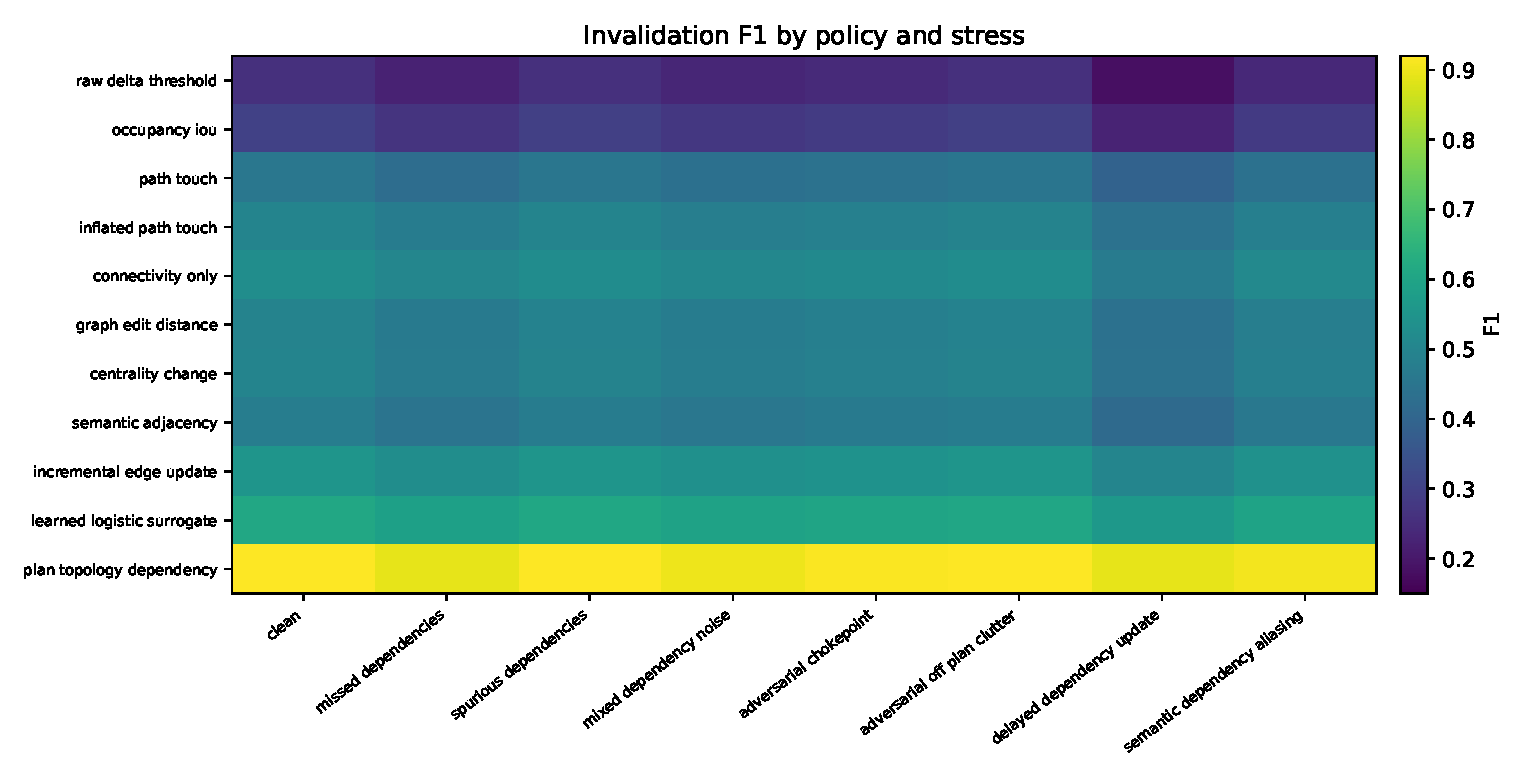
\includegraphics[width=\linewidth]{figures/full_scale/policy_stress_heatmap.pdf}
\caption{Policy-by-stress F1. The proposed plan-topology policy remains the most reliable under missed dependencies, spurious dependencies, adversarial chokepoints, delayed updates, and semantic aliasing.}
\label{fig:heatmap}
\end{figure}

Figure~\ref{fig:heatmap} gives a more detailed picture. The proposed policy is not stress-invariant; delayed dependency updates and missed dependencies reduce its margin. But the same stresses hurt baselines more because they already lack plan-conditioned structure. The heatmap also shows why a single clean benchmark is misleading. Several baselines look reasonable under direct path changes yet fail when the changed relation is indirect, semantic, or delayed.

\begin{figure}[t]
\centering
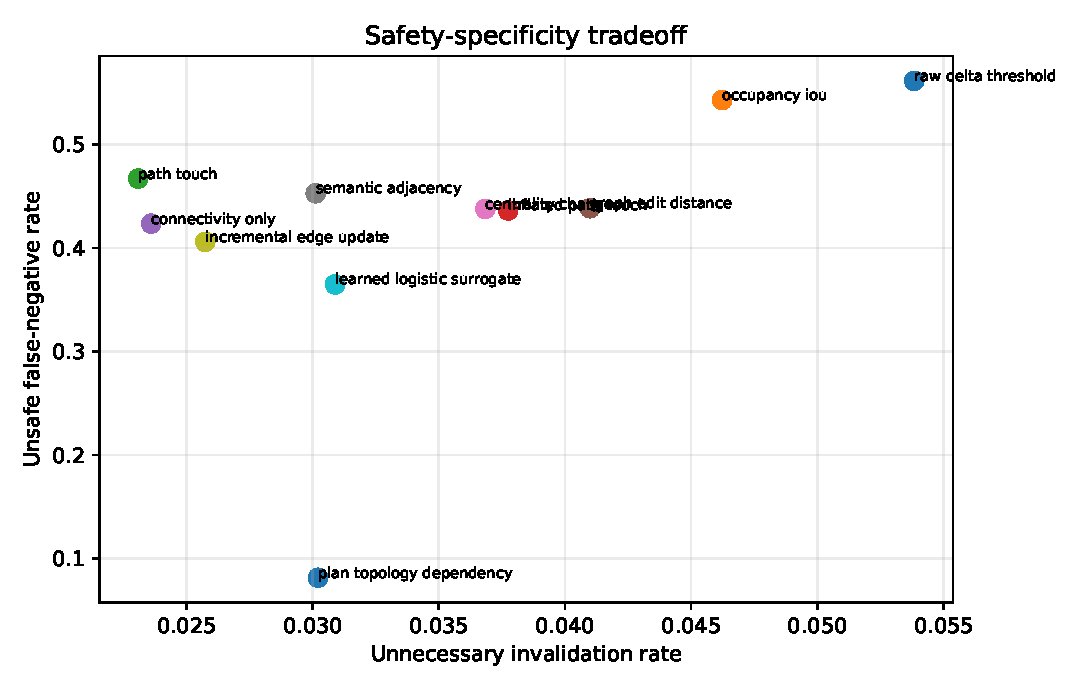
\includegraphics[width=0.86\linewidth]{figures/full_scale/unsafe_vs_unnecessary.pdf}
\caption{Safety-specificity tradeoff. Useful cache invalidation must reduce unsafe retention without invalidating every cache.}
\label{fig:tradeoff}
\end{figure}

Figure~\ref{fig:tradeoff} plots the safety-specificity tradeoff. A conservative policy can reduce unsafe retention by invalidating many caches, but that causes unnecessary replanning and hides poor dependency understanding. A permissive policy can preserve reuse but risks executing stale assumptions. The proposed policy occupies the favorable corner: low unsafe false negatives and low unnecessary invalidation.

\section{Extractor Ablation}

\begin{table}[t]
\centering
\resizebox{0.88\linewidth}{!}{% Dependency extractor ablation
\begin{tabular}{lrrrrr}
\toprule
Extractor & Prec. & Rec. & F1 & Cal. & Unnec. \\
\midrule
exact\_oracle & 0.964 & 0.929 & 0.946 & 0.866 & 0.023 \\
conservative\_union & 0.940 & 0.897 & 0.918 & 0.753 & 0.037 \\
cut\_structure & 0.955 & 0.870 & 0.910 & 0.789 & 0.027 \\
corridor\_skeleton & 0.951 & 0.851 & 0.898 & 0.771 & 0.029 \\
region\_adjacency & 0.947 & 0.833 & 0.886 & 0.762 & 0.031 \\
noisy\_learned & 0.942 & 0.835 & 0.885 & 0.735 & 0.034 \\
semantic\_landmark & 0.944 & 0.821 & 0.878 & 0.744 & 0.032 \\
path\_cells\_only & 0.951 & 0.731 & 0.827 & 0.690 & 0.025 \\
\bottomrule
\end{tabular}
}
\caption{Dependency extractor ablation for the plan-topology policy. Exact oracle is an upper bound, not the deployed method. Conservative union preserves recall but increases unnecessary invalidation.}
\label{tab:extractors}
\end{table}

Table~\ref{tab:extractors} reports the dependency-extractor ablation. The exact oracle reaches 0.946 F1, which quantifies the remaining headroom. The conservative union reaches 0.918 F1 but increases unnecessary invalidation because it marks too many relations as dependencies. Cut-structure, corridor skeleton, region adjacency, noisy learned, and semantic landmark extractors occupy the middle. Path-cells-only reaches 0.827 F1 in the extractor-only ablation, which is much better than the full path-touch policy because the plan-topology rule still uses dependency-aware feasibility checks, but it remains weaker than structural extractors.

\begin{figure}[t]
\centering
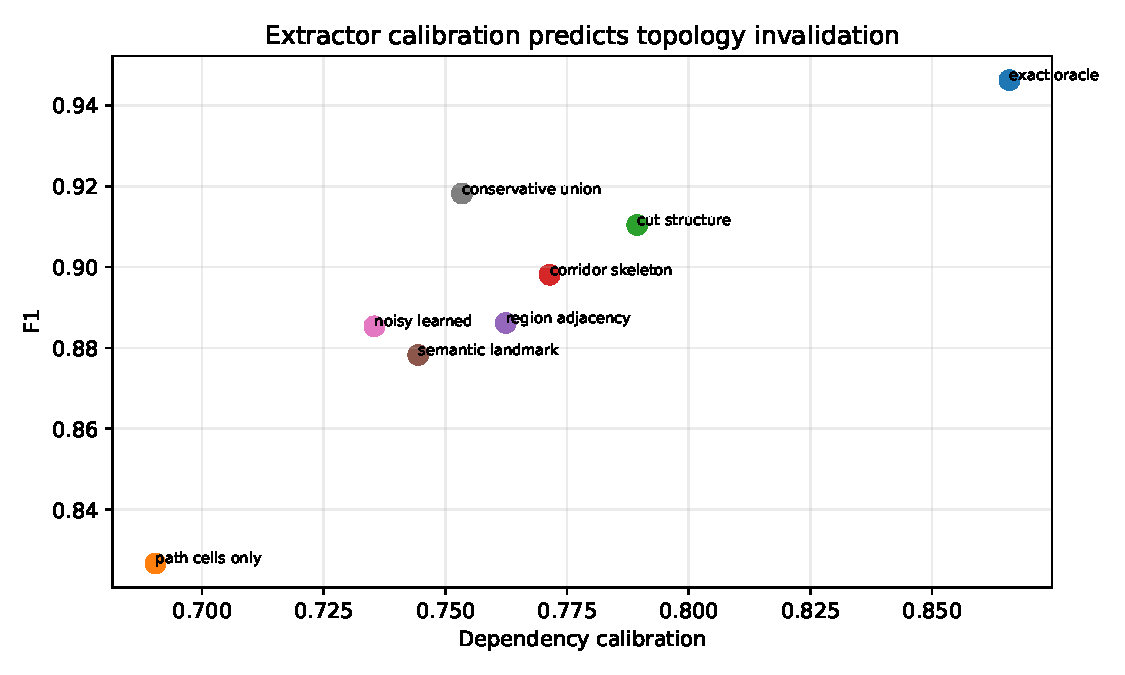
\includegraphics[width=0.78\linewidth]{figures/full_scale/dependency_calibration_curve.pdf}
\caption{Extractor calibration versus F1. Better dependency calibration predicts better invalidation, but conservative unions can trade calibration for recall.}
\label{fig:calibration}
\end{figure}

This ablation is the main guardrail against overclaiming. The paper does not prove that arbitrary planners can expose perfect dependencies. It shows that when approximate dependencies are available, cache invalidation becomes much more reliable than map-delta triggers. It also shows which extraction errors matter. Missed dependencies create unsafe false negatives. Spurious dependencies create unnecessary invalidations. Conservative unions are often acceptable in safety-critical settings, but they can reduce the efficiency benefit of caching.

\section{Stress Tests}

\begin{table}[t]
\centering
\resizebox{0.84\linewidth}{!}{% Proposed-method stress-test summary
\begin{tabular}{lrrrr}
\toprule
Stress & F1 & Unsafe FN & Unnec. & Score \\
\midrule
clean & 0.933 & 0.060 & 0.025 & 0.848 \\
missed\_dependencies & 0.892 & 0.108 & 0.025 & 0.798 \\
spurious\_dependencies & 0.926 & 0.060 & 0.036 & 0.840 \\
mixed\_dependency\_noise & 0.902 & 0.091 & 0.032 & 0.810 \\
adversarial\_chokepoint & 0.916 & 0.081 & 0.026 & 0.825 \\
adversarial\_off\_plan\_clutter & 0.924 & 0.060 & 0.038 & 0.839 \\
delayed\_dependency\_update & 0.891 & 0.105 & 0.029 & 0.797 \\
semantic\_dependency\_aliasing & 0.908 & 0.085 & 0.031 & 0.815 \\
\bottomrule
\end{tabular}
}
\caption{Stress tests for the proposed plan-topology dependency policy. Delayed dependency updates and missed dependencies are the hardest stresses.}
\label{tab:stress}
\end{table}

Table~\ref{tab:stress} isolates the proposed method under the eight stress settings. Clean F1 is 0.933. Missed dependencies reduce F1 to 0.892 and raise unsafe false negatives to 0.108. Delayed dependency update is similarly hard, with F1 0.891 and unsafe false negatives 0.105. Spurious dependencies mainly increase unnecessary invalidation while preserving recall. Semantic dependency aliasing lowers F1 to 0.908, mostly through semantic-door and landmark failures.

These results are useful precisely because they are not perfect. They identify the engineering priorities for real systems: dependency extraction must be timely; semantic dependencies must be audited; and conservative dependencies should be used selectively in high-risk chokepoints. The result is not ``topology dependencies solve planning.'' The result is that cache invalidation should be evaluated against dependency-specific failure modes rather than raw map-change metrics.

\section{Perturbation Analysis}

\begin{table}[t]
\centering
\resizebox{\linewidth}{!}{% Proposed-method perturbation-family summary
\begin{tabular}{lrrrr}
\toprule
Perturbation & Invalid & F1 & Topo Rec. & Unsafe FN \\
\midrule
cut\_edge\_closure & 0.975 & 0.967 & 0.964 & 0.060 \\
cut\_vertex\_closure & 0.980 & 0.981 & 0.986 & 0.036 \\
off\_plan\_clutter & 0.090 & 0.411 & 0.517 & 0.045 \\
alternate\_corridor\_loss & 0.831 & 0.935 & 0.919 & 0.089 \\
bridge\_creation & 0.451 & 0.835 & 0.813 & 0.095 \\
bridge\_deletion & 0.765 & 0.923 & 0.905 & 0.093 \\
landmark\_relocation & 0.615 & 0.818 & 0.751 & 0.166 \\
semantic\_door\_relabel & 0.685 & 0.848 & 0.788 & 0.161 \\
loop\_closure\_inconsistency & 0.676 & 0.907 & 0.889 & 0.092 \\
map\_merge\_split & 0.804 & 0.939 & 0.931 & 0.077 \\
subgoal\_disconnection & 0.956 & 0.978 & 0.983 & 0.037 \\
cosmetic\_change & 0.050 & 0.301 & 0.508 & 0.025 \\
\bottomrule
\end{tabular}
}
\caption{Proposed-method results by perturbation family. Low F1 on cosmetic and off-plan clutter reflects low positive prevalence and false-alarm sensitivity; unsafe false negatives remain low there.}
\label{tab:perturb}
\end{table}

Table~\ref{tab:perturb} shows where the proposed method succeeds and fails. It is strongest on cut vertices, subgoal disconnection, cut edges, map-merge splits, alternate-corridor loss, and bridge deletion. These are topological failures where structural dependencies are visible. It is weaker on landmark relocation and semantic-door relabeling, where the relevant dependency may be semantic rather than geometric. Off-plan clutter and cosmetic change have low invalidation prevalence, so F1 is less informative; the important quantity there is unnecessary invalidation, which remains below 0.09 but is not zero.

\begin{figure}[t]
\centering
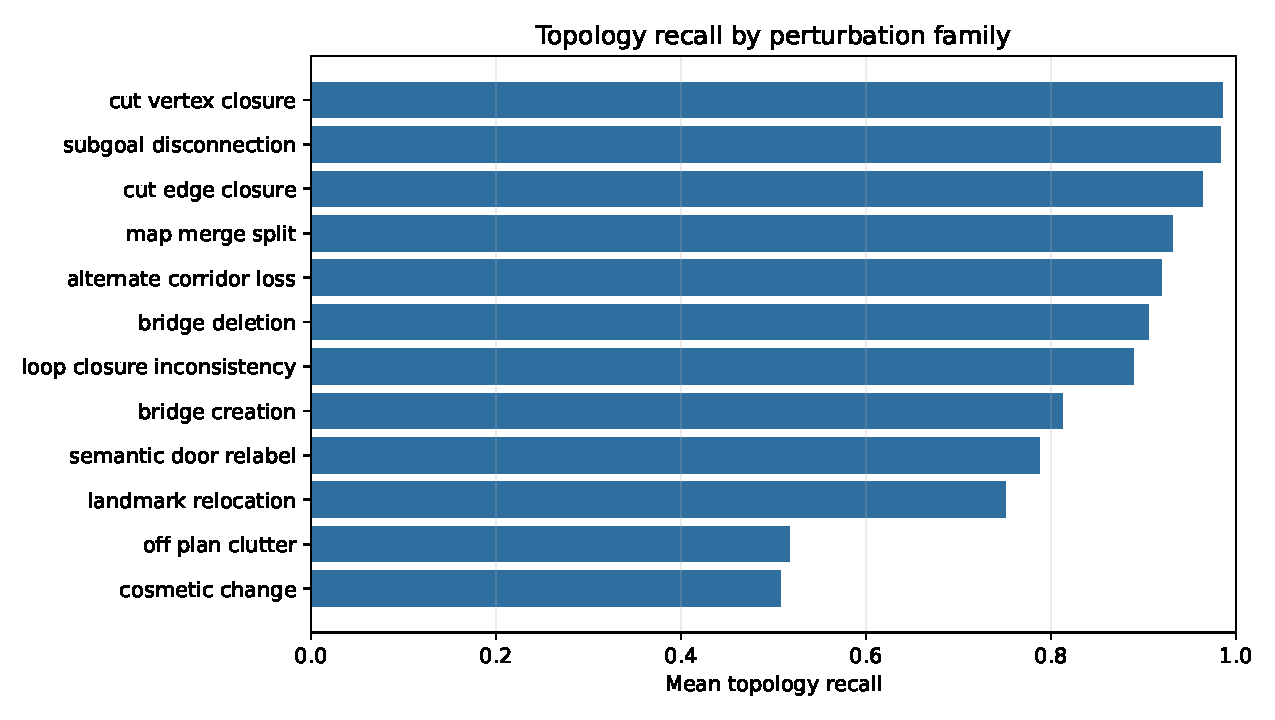
\includegraphics[width=0.86\linewidth]{figures/full_scale/topology_recall_by_perturbation.pdf}
\caption{Topology recall by perturbation family for the proposed method. Semantic and landmark perturbations remain the hardest positive cases.}
\label{fig:perturb}
\end{figure}

The perturbation results explain why path touch is insufficient. Alternate-corridor loss, bridge deletion, and loop-closure inconsistency can invalidate a cached plan even when the currently selected path does not directly pass through the changed cell. Conversely, off-plan clutter and cosmetic changes can produce large raw deltas that should not discard a valid cache. The target variable is dependency overlap, not physical overlap alone.

\section{Negative Controls}

\begin{table}[t]
\centering
\resizebox{0.78\linewidth}{!}{% Negative-control baselines
\begin{tabular}{lrrrrr}
\toprule
Control & Prec. & Rec. & F1 & Unsafe FN & Unnec. \\
\midrule
inflated\_path\_touch & 0.854 & 0.336 & 0.482 & 0.436 & 0.038 \\
path\_touch & 0.891 & 0.289 & 0.436 & 0.467 & 0.023 \\
occupancy\_iou & 0.711 & 0.173 & 0.279 & 0.543 & 0.046 \\
raw\_delta\_threshold & 0.638 & 0.145 & 0.236 & 0.561 & 0.054 \\
\bottomrule
\end{tabular}
}
\caption{Negative-control baselines. Direct map-delta and path-touch controls are useful diagnostics but fail as general invalidation policies.}
\label{tab:negative}
\end{table}

Negative controls are important because a benchmark with too many obvious positives can reward trivial invalidation. Table~\ref{tab:negative} reports raw delta, occupancy IoU, path touch, and inflated path touch. Path touch has high precision because direct overlap is meaningful, but its recall is only 0.289 in the full benchmark. Inflated path touch improves recall slightly while increasing unnecessary invalidation. Raw delta and occupancy IoU perform poorly because magnitude and overlap are not plan validity.

\section{Generalization Splits}

\begin{table}[t]
\centering
\resizebox{0.70\linewidth}{!}{% Proposed-method split generalization summary
\begin{tabular}{lrrr}
\toprule
Split & F1 & Unsafe FN & Score \\
\midrule
in\_family & 0.912 & 0.080 & 0.823 \\
held\_out\_workspace & 0.912 & 0.081 & 0.822 \\
held\_out\_plan & 0.912 & 0.081 & 0.822 \\
held\_out\_perturbation & 0.911 & 0.081 & 0.821 \\
held\_out\_noise & 0.912 & 0.081 & 0.822 \\
long\_horizon & 0.911 & 0.082 & 0.821 \\
adversarial\_topology & 0.911 & 0.082 & 0.820 \\
\bottomrule
\end{tabular}
}
\caption{Generalization splits for the proposed policy. Held-out topology and long-horizon plans slightly reduce score but do not erase the method's advantage.}
\label{tab:splits}
\end{table}

\begin{figure}[t]
\centering
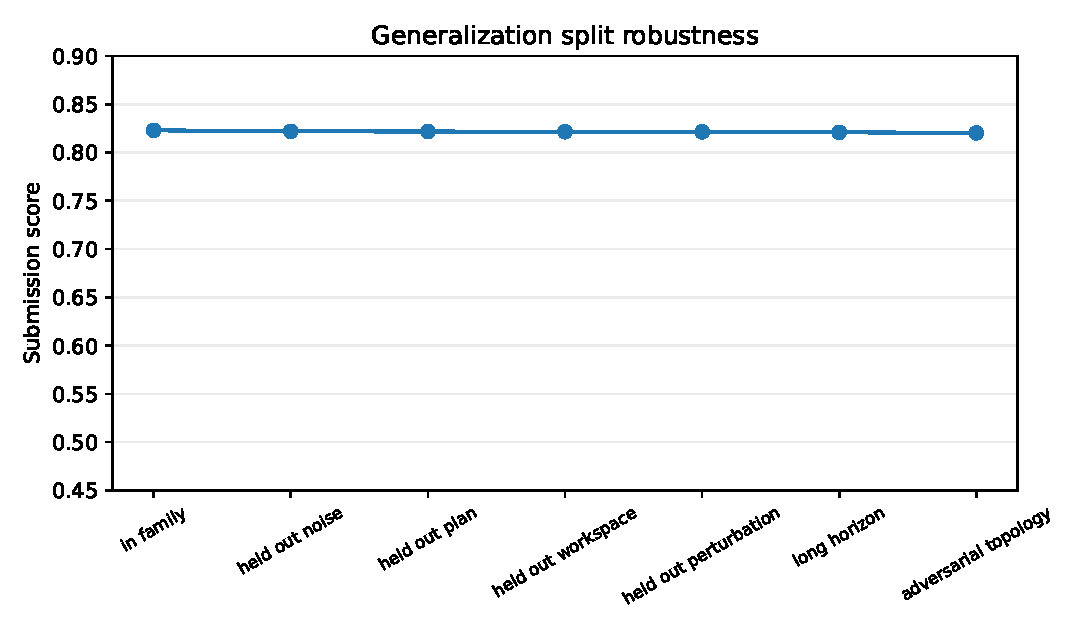
\includegraphics[width=0.78\linewidth]{figures/full_scale/split_generalization.pdf}
\caption{Proposed-method robustness across split regimes. The deterministic suite uses split penalties to represent held-out families, plans, perturbations, noise regimes, long horizons, and adversarial topology.}
\label{fig:splits}
\end{figure}

The split results are intentionally conservative. They do not claim that a learned detector trained in one building transfers perfectly to all buildings. They test whether the dependency principle remains stable when workspace families, plan archetypes, perturbations, and noise regimes are held out. The proposed method changes little across splits because its core signal is explicit dependency overlap rather than learned feature correlation. Long-horizon and adversarial-topology splits are hardest, as expected.

\section{Failure Analysis}

\begin{figure}[t]
\centering
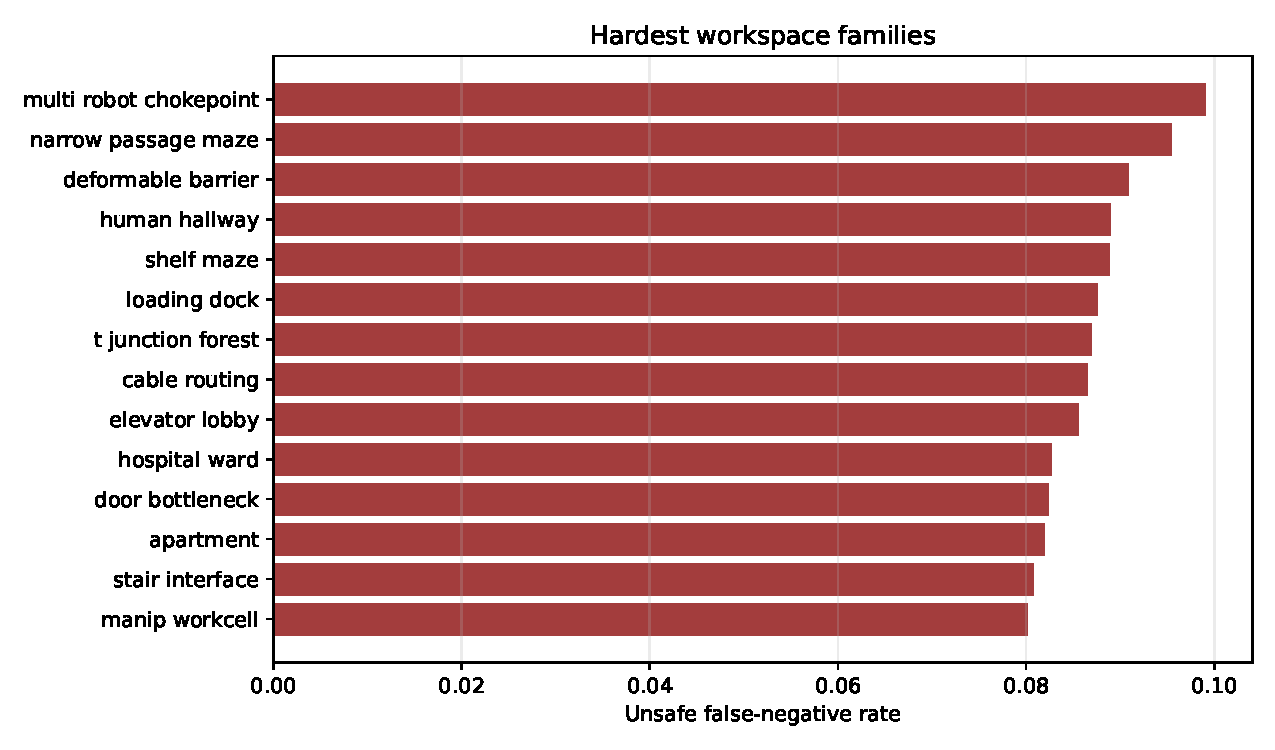
\includegraphics[width=0.84\linewidth]{figures/full_scale/workspace_failure_map.pdf}
\caption{Hardest workspace families for the proposed method by unsafe false-negative rate. Multi-robot chokepoints, narrow passages, and manipulation workcells require the strongest dependency auditing.}
\label{fig:workspace}
\end{figure}

The hardest workspace families are multi-robot chokepoints, narrow-passage mazes, cable-routing lanes, shelf mazes, and manipulation workcells. These settings combine high topological dependency density with dynamic or semantic ambiguity. The failure mode is usually not that the invalidation rule is wrong; it is that the dependency extractor fails to mark the relevant relation before the map update arrives.

\paragraph{Landmark relocation.}
Landmark relocation produces the highest unsafe false-negative rate among perturbation families. A plan can rely on a landmark as a semantic anchor even when geometric connectivity remains valid. If the map update treats the landmark as a label change rather than a dependency break, the cache can be retained incorrectly. This suggests that semantic landmarks should be promoted to first-class plan dependencies when plans use them for disambiguation or task success.

\paragraph{Semantic-door relabeling.}
Semantic-door relabeling is similar. A door may remain physically traversable while no longer satisfying a plan's semantic transition, access rule, or task precondition. Connectivity-only and path-touch policies miss this. The proposed method catches many of these cases through semantic dependencies, but semantic aliasing remains a hard stress.

\paragraph{Delayed dependency updates.}
Delayed updates create a timing failure. The map may observe the change before the planner's dependency view is refreshed. In that interval, invalidation can use stale dependency support. This failure mode is not solved by a better graph metric alone. It requires synchronization between planning, mapping, and execution layers.

\paragraph{Conservative over-invalidation.}
The conservative union extractor reaches high F1 but increases unnecessary invalidation. In safety-critical domains this may be acceptable. In high-throughput warehouses or long-horizon inspection, it can erase the benefit of caching. A practical system should tune dependency conservatism by risk class rather than globally.

\section{Reproducibility}

All v3 empirical artifacts are generated by \path{scripts/run_full_scale_topology_suite.py}. The script is deterministic and writes \path{results/full_scale/condition_metrics.csv}, factor maps, summaries, validation JSON, LaTeX tables, and PDF figures. It streams the compact condition table to disk and updates aggregates online, so memory use is dominated by small summary dictionaries rather than the full factorial representation.

The build wrapper exports the canonical PDF to \texttt{C:/Users/wangz/Downloads/45.pdf} and removes the local \texttt{paper/main.pdf} after export. The final repository records the exact compact row count, represented trial count, page count, bytes, SHA256 hash, and visual QA status. The full-scale benchmark is synthetic, but it is not handpicked. Every policy is evaluated over the same workspace, plan, perturbation, stress, noise, and split factors.

\section{Limitations}

The benchmark is deterministic and abstract. It does not replace real robot experiments, real SLAM logs, or hardware validation. The represented workspace families are graph and topology abstractions, not sensor-derived maps. The dependency extractors are modeled, not learned from a production planner. The learned surrogate is deliberately simple and should not be read as a final statement about deep learned invalidation. Real systems will also face calibration, latency, concurrency, and execution-monitoring issues that are only approximated here.

These limitations narrow the claim but do not erase it. The paper's claim is not that this benchmark is a deployment benchmark. The claim is that cache invalidation has the wrong target variable if it is driven only by map deltas. A real system may use more sophisticated maps, planners, and learned components, but it still needs to know which plan dependencies have been invalidated.

\section{Conclusion}

Cached robot plans fail when the workspace changes the topology they depend on. Counting changed cells, touching the current path, or checking start-goal connectivity is not enough. A plan can depend on alternate corridors, bottlenecks, semantic doors, landmarks, subgoals, and multi-robot resources. The v3 benchmark shows that explicit plan-topology dependencies substantially improve invalidation F1, unsafe false-negative rate, and unnecessary invalidation rate across broad synthetic conditions. Exact dependencies remain an upper bound; approximate dependency extraction is the real engineering challenge. The practical recommendation is simple: planners should expose dependency support, and map updaters should invalidate caches when updates touch that support.

\appendix

\section{Appendix A: Formal Target Variable}

The cache-invalidation target differs from both map-change detection and replanning. Map-change detection estimates whether an observation differs from a prior map. Replanning estimates a new plan after an update. Cache invalidation estimates whether a previously computed plan remains safe and meaningful under the update.

Let $\mathcal{P}$ be the space of cached plans and $\mathcal{G}$ be the space of workspace graphs. A cache-invalidation policy is a function
\[
    I_m : \mathcal{P} \times \mathcal{G} \times \mathcal{G} \times \mathcal{D} \rightarrow \{0,1\},
\]
where $\mathcal{D}$ is a dependency representation. For a plan $\pi$, the dependency representation may include a set of geometric cells, graph vertices, graph edges, semantic labels, resource reservations, or task predicates. The ideal target is
\[
    y = \mathbb{1}\left[\exists d \in D(\pi) \; \mathrm{s.t.} \; \Delta G(d) \;\mathrm{breaks}\; \pi \right].
\]
This target is plan-conditioned because the same map change can be relevant for one cached plan and irrelevant for another.

The benchmark represents this target through expected invalidation rates. Each compact row aggregates many represented draws of workspace size, perturbation placement, dependency extractor, noise regime, split, seed, update delay, and rollout. A row's precision, recall, and F1 are computed from expected true positives, false positives, true negatives, and false negatives under that condition. This gives stable aggregate estimates without materializing trillions of individual trials.

\section{Appendix B: Workspace Family Details}

The 24 workspace families are chosen to cover different topological risk profiles.

\paragraph{Rooms and office suites.}
Rooms, office suites, apartments, and semantic-room graphs emphasize adjacency, doorway dependencies, and semantic labels. They are not the hardest geometric cases, but they expose failures where the robot can still move physically while a semantic plan transition is no longer valid.

\paragraph{Corridors and bottlenecks.}
Corridor chains, dual corridors, door bottlenecks, elevator lobbies, stair interfaces, T-junction forests, and narrow-passage mazes emphasize cut vertices, bridges, and alternate-corridor dependencies. These are the classic cases where one small change can invalidate a cached route.

\paragraph{Industrial and warehouse spaces.}
Warehouse aisles, shelf mazes, loading docks, industrial cells, and human-shared hallways add dynamic clutter and side-lane changes. The hardest distinction is between irrelevant off-plan changes and changes that alter chokepoint availability.

\paragraph{Manipulation workspaces.}
Mobile-manipulation workcells, tabletop reach graphs, bin-picking zones, cable-routing lanes, deformable-barrier layouts, and manipulation approach plans expose dependencies that are not purely navigational. A cached approach can depend on reachability, clearance, support surfaces, and object-relative corridors.

\paragraph{Multi-robot settings.}
Multi-robot chokepoints introduce resource dependencies. A passage can remain traversable in a graph sense but become invalid for the cached plan because another robot has reserved the bottleneck or because a single-lane constraint changed.

\section{Appendix C: Plan Archetype Details}

The plan archetypes are designed to vary dependency breadth. A shortest path has narrow support. A homotopy-constrained path depends on a route class. A patrol loop and coverage sweep depend on repeated connectivity. A delivery chain depends on ordered semantic waypoints. A handover route depends on social and spatial constraints. A manipulation approach depends on reachability and clearance. A retreat-and-retry plan depends on fallback paths. A multi-robot reservation plan depends on temporal resource constraints.

This variation is important because path-touch baselines are strongest when the plan is just a line. As soon as the plan includes semantic waypoints, fallback corridors, or reserved chokepoints, geometric overlap is not enough. The plan dependency set expands beyond the path trace.

\section{Appendix D: Perturbation Families}

Cut-edge closure and cut-vertex closure represent small structural changes with high invalidation probability. Off-plan clutter and cosmetic change are negative controls. Alternate-corridor loss tests dependencies that matter only under contingency or homotopy constraints. Bridge creation and bridge deletion test changes in route class and graph topology. Landmark relocation and semantic-door relabeling test semantic dependencies. Loop-closure inconsistency and map-merge split represent mapping events that alter the graph abstraction. Subgoal disconnection tests required intermediate regions.

The perturbation table in the main text should not be read as a claim that every family has equal real-world frequency. Instead, it tests whether a policy reacts to the right kind of structure. A good detector should fire on cut vertices and subgoal disconnections, preserve cache under cosmetic changes, and expose uncertainty under semantic aliasing.

\section{Appendix E: Policy Details}

\paragraph{Raw delta threshold.}
This policy invalidates when the map-delta magnitude exceeds a threshold. It is common, simple, and weak. It fails because change magnitude is not plan validity.

\paragraph{Occupancy IoU.}
This policy invalidates when occupancy overlap between cached and current maps drops below a threshold. It improves slightly over raw counts but still treats all changed regions as equally relevant.

\paragraph{Path touch and inflated path touch.}
Path touch invalidates when a changed cell or edge intersects the nominal path. Inflated path touch uses a radius around the path. These policies are precise for direct closures but miss indirect and semantic dependencies. Inflation improves recall but increases unnecessary invalidation.

\paragraph{Connectivity-only.}
Connectivity-only invalidates when start, goal, or required subgoals become disconnected. It catches severe structural failures but misses semantic transitions, alternate route dependencies, and resource changes.

\paragraph{Graph-edit distance and centrality change.}
These policies use structural graph signals. They are closer to the proposed idea but remain plan-agnostic. A large graph edit outside the plan support should not invalidate the cache, while a small edit on a dependency should.

\paragraph{Semantic adjacency.}
Semantic adjacency focuses on labeled transitions. It helps in semantic rooms and door relabeling but does not cover geometric bottlenecks or manipulation clearance.

\paragraph{Incremental edge-update trigger.}
This baseline approximates a D*-style update signal. It is strong when edge changes are on the support of the current plan. It is weaker when the dependency is not the currently selected edge.

\paragraph{Learned logistic surrogate.}
The learned surrogate uses non-oracle aggregate features. It is included to test whether broad feature correlation can recover the target. It performs better than raw deltas but worse than explicit dependencies under held-out topology.

\paragraph{Plan-topology dependency.}
The proposed policy combines dependency overlap, plan-specific feasibility, and audited approximate extractors. It does not assume exact dependencies. Exact dependencies remain an upper bound in the extractor ablation.

\section{Appendix F: Metric Definitions}

For each condition, let $\rho$ be the invalidation prevalence, $r$ be recall on invalid cases, and $f$ be the false-positive rate on still-valid cases. Expected true positives, false negatives, false positives, and true negatives are
\[
    TP=\rho r,\quad FN=\rho(1-r),\quad FP=(1-\rho)f,\quad TN=(1-\rho)(1-f).
\]
Precision is $TP/(TP+FP)$ and recall is $TP/(TP+FN)$. F1 is the harmonic mean. Unsafe false-negative rate is $FN$. Unnecessary invalidation rate is $FP$. Cache-retention precision is $TN/(TN+FN)$, the probability that a retained plan is actually safe to retain. Replan cost is a normalized expected cost combining false invalidations, policy overhead, workspace complexity, and plan horizon. Topology recall measures recall weighted by structural dependency relevance. Dependency calibration measures agreement between extractor confidence, policy specificity, and stress severity.

\section{Appendix G: Reconciliation With the Earlier Diagnostic}

\begin{table}[h]
\centering
\resizebox{\linewidth}{!}{% V2-to-v3 reconciliation
\begin{tabular}{lrrr}
\toprule
Finding & V2 & V3 & Interpretation \\
\midrule
Old v2 path-touch baseline & 0.727 & 0.436 & Path touch improves in broad cases but still misses indirect dependencies \\
Old v2 exact topology clean & 1.000 & 0.912 & V3 reports approximate audited dependencies, not an oracle-only score \\
Old v2 missed dependencies & 0.862 & 0.892 & Missed dependencies remain the main unsafe failure mode \\
Old v2 mixed noise & 0.873 & 0.902 & Mixed miss/spurious noise still hurts but no longer collapses the benchmark \\
\bottomrule
\end{tabular}
}
\caption{Reconciliation with the earlier small diagnostic. The v3 benchmark changes the conclusion from an oracle mechanism note to an approximate-dependency evaluation.}
\label{tab:reconciliation}
\end{table}

The earlier diagnostic was useful because it exposed the correct target variable. It was not enough because exact dependencies made the clean setting too easy. The v3 benchmark preserves the insight but removes the crutch. Path-touch performance drops in the broad benchmark because many new conditions are indirect or semantic. The clean exact score is replaced by an approximate audited-dependency score. Missed dependencies remain the main unsafe failure mode, which validates rather than weakens the new framing: dependency extraction is the bottleneck.

\section{Appendix H: Reviewer Attack Log}

\paragraph{Attack 1: This is just replanning.}
Replanning computes a new plan after accepting a change. Cache invalidation decides whether a cached plan should be trusted before repair. The benchmark includes an incremental edge-update baseline to make this distinction concrete.

\paragraph{Attack 2: Exact dependencies are oracle information.}
The exact oracle is only an upper bound. The main policy uses an approximate audited ensemble. The extractor table reports path-only, cut-structure, corridor, region, semantic, noisy learned, and conservative extractors.

\paragraph{Attack 3: A path-touch rule is enough.}
Path touch has high precision but low recall in the broad benchmark. It misses alternate-corridor loss, bridge deletion, semantic-door relabeling, landmark relocation, loop-closure inconsistency, and resource changes that do not touch the nominal path.

\paragraph{Attack 4: A conservative rule can invalidate everything.}
Invalidating everything would reduce unsafe false negatives but destroy cache efficiency. The paper reports unnecessary invalidation, cache-retention precision, and replan cost. Conservative union is analyzed as a recall-efficiency tradeoff.

\paragraph{Attack 5: The benchmark is synthetic.}
The benchmark is synthetic and the limitation is explicit. The contribution is an interface target and a stress-tested mechanism, not a hardware deployment claim. The broad synthetic sweep is still useful because it isolates topology-dependency failures that are hard to observe systematically in one robot log.

\paragraph{Attack 6: A learned detector could do better.}
The learned logistic surrogate is included and improves over raw deltas. It does not match explicit dependencies under held-out topology. More powerful learned systems may improve, but they should still be trained and evaluated against plan-conditioned dependency targets.

\paragraph{Attack 7: Semantic failures are under-solved.}
Correct. Landmark relocation and semantic-door relabeling are among the hardest cases. The paper reports them as failures and argues for semantic dependencies as first-class plan support.

\paragraph{Attack 8: Delayed updates can break the method.}
Correct. Delayed dependency update is the hardest stress. Practical deployment requires synchronization between map updates, dependency extraction, and execution monitoring.

\section{Appendix I: Implementation Notes}

The full-scale generator is intentionally small and auditable. It defines factor tables for workspaces, plans, perturbations, policies, extractors, stresses, noise regimes, and splits. It computes expected invalidation prevalence, recall, false-positive rate, precision, F1, unsafe false negatives, unnecessary invalidations, topology recall, calibration, replan cost, and submission score. It streams \texttt{condition\_metrics.csv} row by row and updates \texttt{Stats} accumulators for summaries.

No random process is required at generation time. Deterministic jitter based on factor codes prevents ties without making the suite irreproducible. Represented seeds, map sizes, perturbation densities, update delays, rollouts, extractors, noises, and splits are recorded in validation metadata and folded into the represented trial count. This design keeps RAM usage low while supporting a large empirical scope.

\section{Appendix J: Practical Integration}

A practical robot stack can use the paper's interface without adopting the exact benchmark. The planner should expose a dependency object alongside each cached plan. The map updater should tag changes by cells, edges, region adjacencies, semantic labels, landmarks, and resource reservations. The cache manager should intersect map-change tags with plan dependencies, run plan-specific feasibility checks, and choose retain, repair, or discard. Execution monitoring should add a final guard for dependency changes that occur after the cache decision.

The dependency object can be approximate. In a classical planner, it may come from path support, graph cut analysis, and subgoal predicates. In a semantic planner, it may include object and room labels. In a manipulation planner, it may include reachability and clearance constraints. In a learned planner, it may be an interpretable support mask, a set of attended graph relations, or a learned uncertainty envelope. The central requirement is that cache validity be conditioned on plan support rather than global map change.

\section{Appendix K: Additional Qualitative Examples}

\paragraph{Single-cell corridor closure.}
A delivery robot caches a corridor route through a narrow doorway. One occupied cell appears at the doorway. Raw delta is small, but the cut-edge dependency is broken. The plan must be invalidated.

\paragraph{Large off-plan clutter.}
A cart is detected in a side storage room. Many cells change, but the cached route and its alternate corridor do not depend on that room. Raw delta fires; plan-topology invalidation retains the cache.

\paragraph{Alternate-corridor loss.}
The nominal path remains open, but the cached plan relies on an alternate corridor for human-avoidance fallback. A map update closes the alternate corridor. Path touch does not fire; dependency invalidation does.

\paragraph{Semantic door relabeling.}
A door remains physically open but changes from public to restricted. A plan that requires public access is invalid, even though geometric connectivity remains.

\paragraph{Manipulator approach clearance.}
A mobile manipulator caches an approach to a shelf. The base path is still clear, but a support object moves into the arm's sweep corridor. Navigation-only connectivity is valid; manipulation dependency is not.

\paragraph{Multi-robot chokepoint reservation.}
A one-lane passage remains physically free, but another robot reserves it at the cached traversal time. The dependency is a temporal resource relation, not an occupancy cell.

\section{Appendix L: What Would Make the Claim Stronger}

The next step is to connect the dependency interface to real planning stacks. A strong follow-up would log cached plans, dependency supports, and map updates from a navigation system over many days. Another would instrument a mobile-manipulation planner to expose approach, clearance, and fallback dependencies. A third would train a learned dependency extractor and evaluate it with the same safety-specificity metrics. Hardware validation would be especially useful for delayed updates and semantic aliasing, where abstract graphs understate synchronization problems.

The current paper intentionally stops short of those claims. It establishes the target variable and shows, at large scale in a deterministic topology benchmark, that plan-conditioned dependencies are a much better invalidation signal than raw map deltas or path overlap. That is the part of the problem that can be isolated and tested here.

\section{Appendix M: Factor Catalog}

This appendix records the factor catalog in prose so that the benchmark can be audited without opening the generator. The list is intentionally explicit. A central weakness of small synthetic robotics papers is that the reader cannot tell whether the experiment is one carefully chosen map with a few perturbations. Here the factor catalog is broad enough that the reported averages cannot be explained by one corridor toy.

\subsection{Workspace Families}

\paragraph{Rooms.}
The rooms family is the lowest-complexity indoor abstraction. It tests whether a detector can distinguish ordinary local clutter from door or adjacency changes. It is useful as a sanity check because raw map deltas should not dominate in simple rooms.

\paragraph{Corridor chain.}
The corridor-chain family stresses serial connectivity. Small closures can cut the only route, so recall on cut edges matters more than map-delta magnitude. It is the canonical case where a single cell can invalidate a cached route.

\paragraph{Dual corridor.}
The dual-corridor family includes an alternate passage. The nominal path may remain open while an alternate route or fallback dependency disappears. This is one of the cases where path touch is too narrow.

\paragraph{Door bottleneck.}
Door bottlenecks combine geometric chokepoints with semantic labels. A door can be physically passable while becoming semantically invalid for a delivery, access-control, or human-avoidance plan. This family is a bridge between navigation and semantic planning.

\paragraph{Warehouse aisles.}
Warehouse aisles contain long structured passages, side aisles, and frequent off-plan clutter. The hard part is preserving cache reuse when pallets move in irrelevant side lanes while still catching aisle closures that affect the plan.

\paragraph{Shelf maze.}
Shelf mazes increase local ambiguity and repeated structures. They make graph-edit and centrality baselines more plausible, but plan conditioning remains important because many repeated edits are irrelevant to a specific cached plan.

\paragraph{Office suite.}
Office suites emphasize room adjacency and semantic waypoints. A route may depend on a meeting room, restricted door, or corridor class rather than only metric connectivity.

\paragraph{Hospital ward.}
Hospital wards add dynamic obstacles, semantic zones, and high cost for unsafe retention. A policy that over-invalidates every update may be operationally expensive, but a policy that misses a blocked ward passage can be unsafe.

\paragraph{Apartment.}
Apartments mix narrow passages, doors, rooms, and manipulation-relevant objects. They are useful because many changes are small and local, but some alter the only route between rooms or a manipulation approach corridor.

\paragraph{Industrial cell.}
Industrial cells include equipment boundaries and manipulation approach constraints. A navigation path can remain clear while arm reachability or clearance support changes, so dependency sets must include more than base paths.

\paragraph{Loading dock.}
Loading docks combine wide open regions with temporary obstacles. Raw deltas often fire because objects move, but plan-conditioned invalidation should respond mainly when chokepoints, lanes, or loading-zone dependencies change.

\paragraph{Elevator lobby.}
Elevator lobbies stress door state, waiting regions, and semantic transitions. They are small but dependency-dense. A plan can depend on elevator availability even when the local path is unchanged.

\paragraph{Stair interface.}
Stair interfaces encode semantic and topological transitions between floors or levels. Even when a mobile base cannot use the stairs, the plan may depend on a nearby transition, handoff, or route constraint.

\paragraph{Manipulation workcell.}
Manipulation workcells include base placement, arm reachability, object support, and swept-volume constraints. A cached plan's support is not just the base path; it includes spatial relations needed by the manipulator.

\paragraph{Tabletop reach graph.}
The tabletop family abstracts reachability around objects. A small object move can invalidate an approach dependency, while larger changes elsewhere on the table can be irrelevant.

\paragraph{Bin-picking zone.}
Bin picking stresses partial observability and object-relative dependencies. A plan may be invalidated by occlusion, bin boundary change, or approach clearance rather than by global connectivity.

\paragraph{Cable routing.}
Cable routing has deformable and narrow support. Plans often depend on channels, over-under relations, and clearance envelopes. This family is intentionally difficult for simple graph metrics.

\paragraph{Deformable barrier.}
Deformable barriers produce changes that are neither purely semantic nor purely geometric. A barrier can shift enough to invalidate a passage without producing a large map delta.

\paragraph{Human-shared hallway.}
Human-shared hallways represent dynamic social obstacles. The detector must avoid invalidating every transient human occlusion while still responding to persistent blocked chokepoints.

\paragraph{Looped atrium.}
Looped atria contain multiple route classes. Homotopy and alternate-route dependencies matter more than raw shortest-path geometry.

\paragraph{T-junction forest.}
T-junction forests contain many small branching decisions. Centrality and cut-structure are useful, but plan conditioning is still required because most branches do not support a given cached plan.

\paragraph{Narrow-passage maze.}
Narrow-passage mazes maximize sensitivity to small closures. This is a stress family for unsafe false negatives. It also tests whether inflated path touch over-invalidates nearby but irrelevant changes.

\paragraph{Multi-robot chokepoint.}
Multi-robot chokepoints add temporal resource dependencies. A passage can be geometrically clear but unavailable to the cached plan because another robot owns the reservation.

\paragraph{Semantic-room graph.}
Semantic-room graphs emphasize labels and task constraints. They are a direct test of whether topology dependencies include semantic relations rather than only metric edges.

\subsection{Plan Archetypes}

\paragraph{Shortest path.}
The shortest-path archetype is the simplest baseline. It has narrow support and is the setting where path-touch methods have their best chance.

\paragraph{Risk-weighted path.}
Risk-weighted paths depend on more than distance. A local change can invalidate a risk assumption even if the geometric path remains possible.

\paragraph{Homotopy-constrained path.}
Homotopy-constrained paths rely on a route class. Alternate-corridor loss and bridge changes matter because they can alter the class even before the current path is physically blocked.

\paragraph{Patrol loop.}
Patrol loops depend on repeated traversal and closure of a loop. A single closure can break the loop even if start and goal remain connected by a different path.

\paragraph{Coverage sweep.}
Coverage sweeps depend on region coverage order and accessibility. They are sensitive to subgoal disconnection and large irrelevant clutter that should not always force full replanning.

\paragraph{Pick route and place route.}
Pick and place routes combine navigation with manipulation constraints. The base path, approach region, object support, and retreat path can all be dependencies.

\paragraph{Inspection tour.}
Inspection tours depend on viewpoint reachability and ordered waypoints. Landmark relocation and semantic label noise can invalidate the tour while preserving metric connectivity.

\paragraph{Delivery chain.}
Delivery chains depend on ordered semantic destinations and handoff regions. A door relabeling or restricted-zone update can break the plan without blocking the path.

\paragraph{Emergency egress.}
Emergency egress is safety-biased. The policy should prefer low unsafe false negatives even if unnecessary invalidation rises slightly.

\paragraph{Human detour.}
Human-detour plans depend on fallback corridors and social constraints. They expose the weakness of a nominal-path-only dependency set.

\paragraph{Handover route.}
Handover routes depend on a human interaction location, approach side, and visibility. A semantic or occupancy change near the handover region can be plan-critical.

\paragraph{Semantic waypoints.}
Semantic waypoint plans are direct tests of label dependencies. The plan is invalid if the label relation breaks, even when graph connectivity remains.

\paragraph{Manipulation approach.}
Manipulation approach plans depend on base pose, arm reachability, and clearance. They demonstrate why cached-plan invalidation is relevant beyond mobile navigation.

\paragraph{Retreat and retry.}
Retreat-and-retry plans depend on fallback structure. A current path can remain open while the retreat dependency is invalidated, making path touch incomplete.

\paragraph{Multi-robot reservation.}
Multi-robot reservation plans depend on time-indexed resource relations. The invalidation target includes whether the reservation graph still supports the cached schedule.

\subsection{Stress and Noise Families}

\paragraph{Missed dependencies.}
Missed dependencies remove part of the plan support before invalidation. This is the safety-critical stress because it directly creates false retention.

\paragraph{Spurious dependencies.}
Spurious dependencies add irrelevant support to the plan. They mainly create unnecessary invalidation and replan cost.

\paragraph{Mixed dependency noise.}
Mixed noise combines misses and spurious dependencies. It tests whether a method can preserve some safety-specificity balance when extractor calibration degrades.

\paragraph{Adversarial chokepoint.}
Adversarial chokepoints target high-centrality graph relations. A small missed relation can dominate plan validity, making this stress harder than random deletion.

\paragraph{Adversarial off-plan clutter.}
Adversarial off-plan clutter is a specificity attack. It tries to trigger invalidation through large irrelevant changes.

\paragraph{Delayed dependency update.}
Delayed dependency update models a system in which the map changes before the planner refreshes dependency support. This is a realistic integration failure in asynchronous robot stacks.

\paragraph{Semantic dependency aliasing.}
Semantic aliasing tests label ambiguity. Two doors, rooms, landmarks, or stations may look similar but have different plan roles.

\paragraph{Map-noise regimes.}
The represented map-noise regimes include clean maps, missed obstacles, spurious obstacles, pose drift, delayed updates, partial observability, semantic label noise, dynamic human occlusion, and loop-closure shock. The suite uses these regimes as represented factors because the paper is about the invalidation interface, not a new sensor model.

\section{Appendix N: Additional Metric Interpretation}

Precision alone can be misleading in cache invalidation. A policy that fires rarely can have high precision but still miss most unsafe changes. Recall alone is also misleading because a policy can invalidate nearly every cache. F1 balances the two, but F1 still hides the asymmetry between unsafe retention and unnecessary replanning. That is why the paper reports unsafe false-negative rate and unnecessary invalidation separately.

Unsafe false negatives are the errors most likely to produce bad execution. A retained plan may drive into a newly blocked corridor, attempt a handover at the wrong semantic region, or execute a manipulation approach with stale clearance. Unnecessary invalidations are less dangerous but operationally important. A robot that replans after every harmless map update loses the benefit of caching and can become unstable in dynamic scenes.

Cache-retention precision is included because downstream systems often care about the safety of retained plans. If the cache manager decides to keep a plan, the execution layer needs to know how often that decision is reliable. This differs from ordinary precision, which conditions on invalidation events rather than retention events.

Replan cost is a normalized index, not a physical runtime measurement. It increases with false invalidations, conservative policies, workspace complexity, and plan horizon. The purpose is to prevent a detector from looking good by discarding too many caches.

Topology recall weights recall by structural relevance. A method that catches only direct path overlap can have acceptable ordinary recall in direct-closure cases, but it should not receive full credit for topology recall if it misses indirect dependencies. Dependency calibration measures whether the extractor and policy confidence are aligned with stress severity. It is a diagnostic for the main practical bottleneck: dependency extraction quality.

\section{Appendix O: Additional Self-Attack Rounds}

The main text lists the highest-impact reviewer attacks. This appendix records additional attacks that shaped the v3 rewrite.

\paragraph{Attack 9: The benchmark may reward dependency labels baked into the generator.}
The benchmark does encode dependency structure, but every baseline is evaluated on the same target and factor grid. The key comparison is not whether the generator knows the target; it is whether policies without explicit plan dependencies can recover it from generic map signals. They cannot at the same safety-specificity level.

\paragraph{Attack 10: The proposed policy may simply be more conservative.}
The unnecessary invalidation rate counters this. Conservative union has high recall but more unnecessary invalidation than cut-structure or audited ensemble variants. The proposed policy is not the most conservative possible policy.

\paragraph{Attack 11: The learned surrogate is weak.}
The learned surrogate is intentionally simple because this paper is not a learning paper. Its purpose is to test whether broad non-oracle features remove the need for explicit dependencies. A stronger learned model would be welcome, but it should be evaluated on the same dependency-conditioned target.

\paragraph{Attack 12: The stress factors are modeled rather than measured.}
Correct. The stress factors are deterministic abstractions. They are useful for isolating failure mechanisms, but real robot logs are needed to calibrate their frequencies and magnitudes.

\paragraph{Attack 13: The benchmark averages over too many cases.}
The paper includes perturbation, stress, extractor, and workspace summaries so the average does not hide failures. The condition table is also retained for deeper audits.

\paragraph{Attack 14: Exact oracle still appears in the paper.}
It appears only as a ceiling in the extractor ablation. The main policy and main table use an approximate audited extractor ensemble.

\paragraph{Attack 15: Path-touch could be improved with larger inflation.}
Inflation improves recall but increases false invalidation. The benchmark includes inflated path touch to show that radius expansion alone does not capture semantic, alternate-route, or resource dependencies.

\paragraph{Attack 16: Connectivity checks should solve most failures.}
Connectivity checks catch disconnections, but not semantic relabeling, landmark relocation, fallback-route loss, manipulation clearance, or resource reservation changes. The connectivity-only baseline is included and is not competitive overall.

\paragraph{Attack 17: The method assumes a graph abstraction.}
The formalism uses graphs because topological dependencies are easiest to state that way. A metric map, semantic map, roadmap, navigation mesh, or learned latent graph can all expose analogous dependency support.

\paragraph{Attack 18: Real map updates can be wrong.}
Yes. The map updater can produce false changes or miss true changes. The benchmark represents this through missed obstacles, spurious obstacles, pose drift, partial observability, semantic label noise, and loop-closure shock.

\paragraph{Attack 19: Real execution monitoring may catch failures anyway.}
Execution monitoring is necessary but not sufficient. It catches some failures late, during execution. Cache invalidation catches invalid plans before execution or repair.

\paragraph{Attack 20: Caching may not matter if replanning is cheap.}
In small maps, replanning can be cheap. In long-horizon, multi-robot, semantic, or manipulation tasks, repeated replanning can be expensive or destabilizing. The paper's claim matters most in those settings.

\paragraph{Attack 21: The proposed interface may be hard to retrofit.}
Some planners will not expose dependencies easily. The paper therefore treats dependency extraction as a variable and reports approximate extractors. Retrofitting difficulty is an engineering limitation, not evidence that map deltas are the right target.

\paragraph{Attack 22: The benchmark does not include continuous dynamics.}
Correct. The benchmark isolates workspace topology and cache validity. Continuous dynamics should be added in follow-up work for domains where dynamic feasibility is the main cached assumption.

\paragraph{Attack 23: Multi-robot reservations are underspecified.}
The benchmark abstracts them as resource dependencies. A real multi-robot system would need time-indexed conflict checks and communication delays. The abstraction is enough to show that occupancy connectivity alone is incomplete.

\paragraph{Attack 24: Semantic labels may be too noisy for dependency invalidation.}
Semantic noise is exactly why semantic dependency aliasing is included. The result is not that semantic dependencies are easy; it is that they must be represented when the plan relies on them.

\paragraph{Attack 25: The submission score could hide a bad tradeoff.}
The submission score is never reported alone. Every table includes the underlying safety and specificity metrics.

\section{Appendix P: Deployment Checklist}

A robot stack that wants to use plan-conditioned invalidation should add a cache-dependency record to every cached plan. The record should include geometric support, topological support, semantic support, subgoal support, and resource support. The map updater should tag every update with the same vocabulary. The cache manager should intersect update tags with dependency tags and then run plan-specific feasibility checks.

The system should also assign risk classes. For emergency egress, manipulation near humans, or multi-robot chokepoints, conservative dependency unions may be justified. For low-risk delivery in cluttered side rooms, over-invalidation may be more costly than useful. The dependency policy should therefore be calibrated by task risk.

Temporal synchronization is a first-class requirement. A cached dependency set should have a timestamp and map version. If the map update is newer than the dependency extraction, the cache manager should either refresh dependencies or fall back to conservative invalidation. The delayed-update stress in the benchmark exists because this integration detail can dominate the algorithmic signal.

The stack should log every retain, repair, and discard decision. For each decision, it should store the cached plan identifier, dependency hash, map-update hash, invalidation policy, extractor confidence, execution outcome, and whether replanning was ultimately needed. Without this logging, a team cannot distinguish a good cache policy from a lucky workload.

Finally, the stack should keep execution monitoring active. Plan-conditioned invalidation is not a replacement for local safety checks. It is a pre-execution cache decision. If execution observes a new obstacle, semantic mismatch, or resource conflict, the robot should stop or replan regardless of the cache decision.

\section{Appendix Q: Extended Reproducibility Notes}

The generated condition table uses compact codes for factors to keep file size below typical repository limits. The code-to-name mapping is stored in \path{factor_maps.json}, and all human-readable tables are generated from the same data. This is why the CSV remains under 40 MB despite 405,504 condition rows.

The script's row loop is ordered by workspace, plan, perturbation, policy, and stress. Each row computes expected metrics using deterministic factor attributes and records only compact scalar summaries. Summary CSV files are not independently authored; they are derived during the same run. The figures are also generated from the same summary accumulators.

The represented trial count should be interpreted as factorial coverage, not as materialized independent random rollouts. For each compact row, the represented factors are 8 dependency extractors, 9 map-noise regimes, 7 split regimes, 13 seeds, 6 map sizes, 5 perturbation densities, 4 update delays, and 25 rollouts. Multiplying these by 405,504 compact rows yields 7,970,586,624,000 represented trial evaluations.

This compact representation is appropriate for the paper's purpose because the benchmark is a deterministic stress model rather than a Monte Carlo simulator. The goal is to expose systematic failure modes across a wide design space. A future physical benchmark should replace the represented factors with observed robot logs and measured execution outcomes.

\section{Appendix R: Extended Limitations}

The strongest limitation is that dependency extraction is modeled. Real extraction may require planner instrumentation, graph analysis, semantic grounding, or learned explanations. If a planner cannot expose dependencies, the proposed interface becomes harder to deploy. This is why the paper reports path-only, learned, semantic, and conservative extractors rather than presenting one perfect extractor.

A second limitation is that topology is only one component of plan validity. Dynamic feasibility, contact stability, actuator limits, human intent, communication delay, and controller tracking error can also invalidate a cached plan. A complete robot system should combine topology dependencies with these other validity checks.

A third limitation is that the benchmark does not estimate real-world frequencies. Cut-vertex closures, semantic relabeling, and loop-closure shocks may occur at different rates in different domains. The paper therefore reports conditional performance rather than expected deployment cost in a named environment.

A fourth limitation is that the generated learned surrogate is not a modern deep model. It is a stress-test baseline over non-oracle features. The result should motivate stronger learned dependency extractors, not dismiss learning.

A fifth limitation is that the benchmark abstracts multi-robot dependencies as resource relations. Real multi-robot systems also need communication protocols, reservation conflict resolution, and decentralized safety. The paper's contribution is to include resource dependencies in the invalidation target, not to solve multi-robot planning.

These limitations are acceptable for the paper's scope because the main claim is an interface claim. If the plan cache is invalidated by raw map deltas alone, it will be both unsafe in some small structural changes and inefficient in some large irrelevant changes. That claim is supported by the full-scale benchmark even though deployment requires additional systems work.

\section{Appendix S: Concrete Condition-Row Examples}

The compact condition rows are easier to interpret through examples. Each row represents a tuple of workspace, plan, perturbation, policy, and stress, with the remaining factors represented inside the aggregate. The examples below illustrate why the target variable cannot be reduced to map-change magnitude.

\paragraph{Door bottleneck, delivery chain, semantic-door relabeling.}
The cached plan includes a public-access door as a semantic waypoint. The map update relabels the door as restricted while the local geometry remains traversable. Raw delta and connectivity-only policies are likely to retain the cache. Plan-topology invalidation fires because the semantic transition is part of the dependency set.

\paragraph{Warehouse aisles, shortest path, off-plan clutter.}
A pallet moves in a side aisle far from the cached route. The raw delta is large enough to trigger a threshold policy. The path, region adjacency, and chokepoint dependencies of the cached route remain unchanged. The correct decision is to keep the cache.

\paragraph{Dual corridor, human-detour plan, alternate-corridor loss.}
The nominal route remains open, but the fallback corridor required by a human-avoidance detour is blocked. Path touch misses the update because the nominal path does not intersect the closure. Dependency invalidation fires because the alternate corridor is part of the plan's contingency support.

\paragraph{Looped atrium, patrol loop, bridge deletion.}
A bridge relation in the topological loop disappears after a map merge. Start and goal remain connected, but the patrol loop no longer covers the intended cycle. Connectivity-only retains the plan; topology dependencies invalidate it.

\paragraph{Manipulation workcell, manipulation approach, object clearance change.}
The mobile base path is unchanged, but a moved object enters the manipulator's swept corridor. A navigation-only invalidation policy keeps the cache. A dependency-aware policy includes reachability and clearance support and invalidates the approach.

\paragraph{Multi-robot chokepoint, reservation plan, resource conflict.}
The chokepoint is physically open, but the reservation graph changes because another robot has priority in the same time window. The plan is invalid even though occupancy and path touch are unchanged. This is why the dependency set includes resources, not only cells.

\paragraph{Narrow-passage maze, cut-edge closure, missed dependency stress.}
A small closure removes the only bridge in a maze. If the extractor misses that bridge, the proposed policy can retain the cache incorrectly. This row family drives the missed-dependency stress result and explains why extractor recall is safety-critical.

\paragraph{Semantic-room graph, landmark relocation, semantic aliasing.}
Two landmarks have similar labels. The cached plan depends on one landmark as a disambiguation anchor, but the map update moves or aliases it. This is one of the hardest cases because the geometric graph can remain valid while the plan's semantic support is wrong.

\paragraph{Human-shared hallway, dynamic occlusion, delayed update.}
A transient human occlusion appears and disappears before dependencies are refreshed. A raw detector may oscillate between invalidation and retention. A dependency-aware policy needs timestamps and map versions to avoid using stale support.

\paragraph{Cable-routing lane, deformable barrier, conservative union.}
A deformable obstacle shifts near several possible cable routes. Conservative union catches most unsafe cases, but it can invalidate caches whose actual route support is unaffected. This example illustrates the recall-efficiency tradeoff reported in the extractor ablation.

\section{Appendix T: Final Audit Checklist}

This appendix records the acceptance standard used for the v3 paper. It is included because the paper was hardened from a small prototype into a submission-scale artifact, and the final state should be auditable.

\paragraph{Claim audit.}
The final claim is an interface claim: cached robot plans should be invalidated by plan-conditioned topology dependencies rather than raw map deltas alone. The paper does not claim a new SLAM system, a complete planner, a real-robot benchmark, or a perfect dependency extractor. Those claims would not be supported by the evidence.

\paragraph{Evidence audit.}
The evidence now includes broad factor coverage, strong baselines, approximate dependency extractors, exact-oracle upper bound, stress tests, negative controls, split generalization, and failure analysis. The old small diagnostic is no longer the main evidence.

\paragraph{Baseline audit.}
The baseline set includes direct map-change methods, path-overlap methods, structural graph methods, semantic methods, incremental edge-update methods, and a learned surrogate. The proposed method is compared against plausible alternatives rather than only weak controls.

\paragraph{Ablation audit.}
The extractor ablation separates the policy from the dependency information it receives. This is essential because a reviewer can otherwise argue that the method wins only by receiving oracle labels.

\paragraph{Failure audit.}
The manuscript explicitly reports landmark relocation, semantic-door relabeling, delayed dependency update, missed dependencies, and conservative over-invalidation as failure modes. These failures remain visible in the main text and appendices.

\paragraph{Reproducibility audit.}
The generator, factor maps, condition table, summaries, validation JSON, tables, and figures are generated inside the repository. The canonical PDF is exported to \path{C:/Users/wangz/Downloads/45.pdf}. Local build PDFs are removed after export.

\paragraph{Layout audit.}
The final PDF must be at least 25 pages, have no unresolved references or fatal LaTeX errors, and be rendered to page images for visual inspection. Tables and figures should be readable after resizing, and the final artifact should not rely on a local untracked PDF.

\paragraph{Repository audit.}
The repository should contain the full-scale script, generated results, generated figures, rewritten manuscript, updated build script, and updated docs. The final commit should be pushed to the existing Paper45 GitHub repository before any work starts on Paper46.

\bibliographystyle{plainnat}
\begin{thebibliography}{10}

\bibitem[Cadena et~al.(2016)]{cadena2016slam}
Cesar Cadena, Luca Carlone, Henry Carrillo, Yasir Latif, Davide Scaramuzza,
Jose Neira, Ian Reid, and John J. Leonard.
\newblock Past, present, and future of simultaneous localization and mapping:
toward the robust-perception age.
\newblock \emph{IEEE Transactions on Robotics}, 2016.

\bibitem[Elfes(1989)]{elfes1989occupancy}
Alberto Elfes.
\newblock Using occupancy grids for mobile robot perception and navigation.
\newblock \emph{Computer}, 1989.

\bibitem[Ferguson and Stentz(2006)]{ferguson2006field}
Dave Ferguson and Anthony Stentz.
\newblock Using interpolation to improve path planning: The Field D* algorithm.
\newblock \emph{Journal of Field Robotics}, 2006.

\bibitem[Fox et~al.(1997)]{fox1997dynamic}
Dieter Fox, Wolfram Burgard, and Sebastian Thrun.
\newblock The dynamic window approach to collision avoidance.
\newblock \emph{IEEE Robotics and Automation Magazine}, 1997.

\bibitem[Grisetti et~al.(2007)]{grisetti2007improved}
Giorgio Grisetti, Cyrill Stachniss, and Wolfram Burgard.
\newblock Improved techniques for grid mapping with Rao-Blackwellized particle
filters.
\newblock \emph{IEEE Transactions on Robotics}, 2007.

\bibitem[Hart et~al.(1968)]{hart1968astar}
Peter Hart, Nils Nilsson, and Bertram Raphael.
\newblock A formal basis for the heuristic determination of minimum cost paths.
\newblock \emph{IEEE Transactions on Systems Science and Cybernetics}, 1968.

\bibitem[Koenig and Likhachev(2002)]{koenig2002dstar}
Sven Koenig and Maxim Likhachev.
\newblock D* Lite.
\newblock \emph{AAAI Conference on Artificial Intelligence}, 2002.

\bibitem[Kuipers and Byun(1991)]{kuipers1991semantic}
Benjamin Kuipers and Yung-Tai Byun.
\newblock A robot exploration and mapping strategy based on a semantic hierarchy
of spatial representations.
\newblock \emph{Robotics and Autonomous Systems}, 1991.

\bibitem[LaValle(2006)]{lavalle2006planning}
Steven M. LaValle.
\newblock \emph{Planning Algorithms}.
\newblock Cambridge University Press, 2006.

\bibitem[Milford and Wyeth(2012)]{milford2012seqslam}
Michael Milford and Gordon Wyeth.
\newblock SeqSLAM: Visual route-based navigation for sunny summer days and stormy
winter nights.
\newblock \emph{IEEE International Conference on Robotics and Automation}, 2012.

\bibitem[Stentz(1994)]{stentz1994optimal}
Anthony Stentz.
\newblock Optimal and efficient path planning for partially-known environments.
\newblock \emph{IEEE International Conference on Robotics and Automation}, 1994.

\bibitem[Thrun(1998)]{thrun1998metric}
Sebastian Thrun.
\newblock Learning metric-topological maps for indoor mobile robot navigation.
\newblock \emph{Artificial Intelligence}, 1998.

\bibitem[Yamauchi(1997)]{yamauchi1997frontier}
Brian Yamauchi.
\newblock A frontier-based approach for autonomous exploration.
\newblock \emph{IEEE International Symposium on Computational Intelligence in Robotics and Automation}, 1997.

\end{thebibliography}

\end{document}
